%%%%%%%%%%%%%%%%%%%%%%%%%%%%%%%%%%%%%%%%%
% University Assignment Title Page 
% LaTeX Template
% Version 1.0 (27/12/12)
%
% This template has been downloaded from:
% http://www.LaTeXTemplates.com
%
% Original author:
% WikiBooks (http://en.wikibooks.org/wiki/LaTeX/Title_Creation)
%
% License:
% CC BY-NC-SA 3.0 (http://creativecommons.org/licenses/by-nc-sa/3.0/)
% 
% Instructions for using this template:
% This title page is capable of being compiled as is. This is not useful for 
% including it in another document. To do this, you have two options: 
%
% 1) Copy/paste everything between \begin{document} and \end{document} 
% starting at \begin{titlepage} and paste this into another LaTeX file where you 
% want your title page.
% OR
% 2) Remove everything outside the \begin{titlepage} and \end{titlepage} and 
% move this file to the same directory as the LaTeX file you wish to add it to. 
% Then add \input{./title_page_1.tex} to your LaTeX file where you want your
% title page.
%
%%%%%%%%%%%%%%%%%%%%%%%%%%%%%%%%%%%%%%%%%
%\title{Title page with logo}
%----------------------------------------------------------------------------------------
%	PACKAGES AND OTHER DOCUMENT CONFIGURATIONS
%----------------------------------------------------------------------------------------

\documentclass[12pt]{article}
% \usepackage[english]{babel}
% \usepackage[utf8x]{inputenc}
\usepackage{amsmath}
\usepackage{graphicx}
\usepackage{listings}
\usepackage{biblatex}
\usepackage{float}
\bibliography{references.bib}
% \usepackage[colorinlistoftodos]{todonotes}
\newtheorem{theorem}{Theorem}


\textheight=250truemm \textwidth=160truemm 
\hoffset=-10truemm \voffset=-30truemm

\begin{document}

\begin{titlepage}

\newcommand{\HRule}{\rule{\linewidth}{0.5mm}} % Defines a new command for the horizontal lines, change thickness here

\center % Center everything on the page
 
%----------------------------------------------------------------------------------------
%	HEADING SECTIONS
%----------------------------------------------------------------------------------------
\vspace*{0.5cm}
\textsc{\LARGE Ukrainian Catholic University}\\[1cm] % Name of your university/college
\textsc{\Large  Faculty of Applied Sciences}\\[0.5cm] % Major heading such as course name
\textsc{\large Data Science Master Program}\\[0.5cm] % Minor heading such as course title

%----------------------------------------------------------------------------------------
%	TITLE SECTION
%----------------------------------------------------------------------------------------
\vspace*{1.5cm}

\HRule \\[0.4cm]
{ \huge \bfseries Agent adaptation to a changing environment}\\[10pt]
{\Large \bfseries Machine Learning Project}\\[0.4cm] % Title of your document
\HRule \\[1cm]
 
%----------------------------------------------------------------------------------------
%	AUTHOR SECTION
%----------------------------------------------------------------------------------------
\vspace*{2.5cm}

\Large \emph{Authors:}\\
Oleg  \textsc{Dats}\\
Dmitri \textsc{Glusco}\\ % Your name

%----------------------------------------------------------------------------------------
%	DATE SECTION
%----------------------------------------------------------------------------------------
\vspace*{0.5cm}
{\large \today}\\[0.5cm] % Date, change the \today to a set date if you want to be precise

%----------------------------------------------------------------------------------------
%	LOGO SECTION
%----------------------------------------------------------------------------------------


\includegraphics[height=5cm]{UCU-Apps.png}\\[0.5cm] % Include a department/university logo - this will require the graphicx package
 
%----------------------------------------------------------------------------------------
% Fill the rest of the page with whitespace

\end{titlepage}
\begin{abstract}
In this project \cite{Project}, we analyze the ability of the Reinforcement Learning (RL) \cite{RL} agent to generalize experience that he receives from the environment.

Research from the "Assessing Generalization in Deep Reinforcement Learning" paper \cite{GeneralizationPaper} was used as a base for this project.

First, the Q-learning \cite{QLearningExplanation} was implemented and applied to FrozenLake environment from OpenAI Gym \cite{OpenAIGym} to learn and experiment with RL approaches. Then Deep Q-Network (DQN) \cite{DQNMedium} from OpenAI Baselines GitHub \cite{OpenAIBaselines} was used to make experiments on the CartPole environments of 3 types: Default (Deterministic), Random and Extreme. CartPole environment was used from Sunblaze environments GitHub \cite{Sunblaze}. Finally, DQN was used to inspect generalization abilities on Pong environment from OpenAI Baselines Atari Wrappers. Noise and pepper were manually added to the environment to simulate Random Environment. DQN was learned on pixel features from the image.

Experiments showed that learning on the Random type of environment increases the learning time, but also increases the performance on Random and Extreme environments improving the ability to generalize.
\end{abstract}
\vspace*{0.8cm}
\section{Introduction}

Nowadays Machine Learning achieved a lot of great not only theoretical but also practical results. Image Classification, Recommender Systems, various NLP applications, time series predictions and etc. And it is still far from the limit. A special place in the Machine Learning tasks takes the goal to explore and build the Artificial General Intelligence (AGI) \cite{AGI}. Currently, AGI is not achieved yet. Reinforcement Learning (RL) \cite{RL} is considered as the closest approach to achieve AGI nowadays. But there is a lot of different problems in the RL to achieve AGI. One of the big problems is that the RL agent tends to overfit.

\section{Reinforcement Learning}

\begin{figure}[H]
\centering
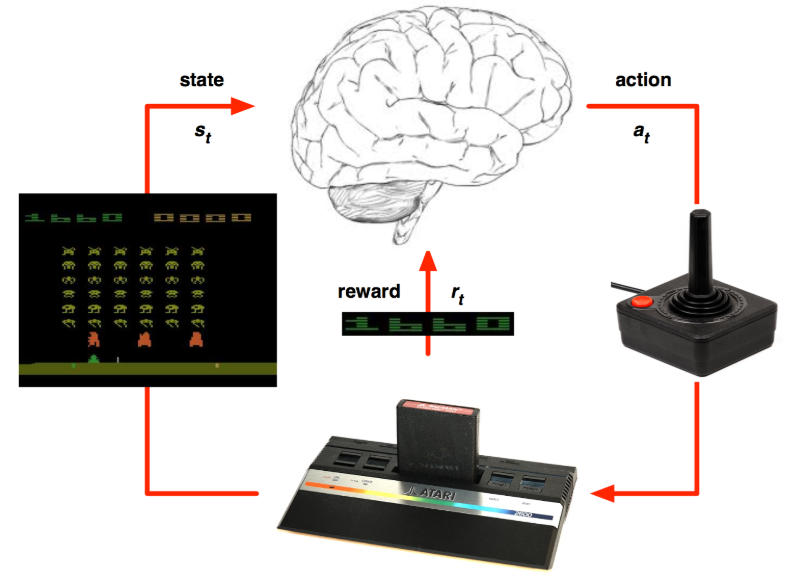
\includegraphics[scale=0.6]{RL_main_idea.png}\\[0.5cm] 
\caption{Agent interaction. Used from DeepMind Youtube video course.}
\end{figure}

In the RL environment agent interacts with the environment and tries to maximize the cumulative reward. Agent receives the state and the reward from the environment and interacts with it using actions.

$R_t$ - \textbf{reward}

$A_t$ - \textbf{action}

$O_t$ - \textbf{observation}

$H_t$ - \textbf{history}. $H_t$ = $A_1,O_1,R_1,\dots,A_t,O_t,R_t$

$S_t$ - \textbf{state} - information used to determine what happens next. $S_t = f(H_t)$

The environment is described as a Markov Decision Process (MDP), that is defined by the $\langle\mathcal{S},\mathcal{A},\mathcal{P},\mathcal{R},\gamma\rangle$, where:
\begin{enumerate}
    \item 
        $\mathcal{S}$ is a (finite) set of states
    \item 
        $\mathcal{A}$ is a (finite) set of actions
    \item
        $\mathcal{P}$ is a state transition probability matrix, $\mathcal{P}^a_{s s'}=\mathbb{P}[S_{t+1}=s'|S_t=s,A_t=a]$
    \item
        $\mathcal{R}$ is a reward function, $\mathcal{R}_s^a=\mathbb{E}[R_{t+1}|S_t=s, A_t=a]$
    \item
        $\gamma$ is a discount factor, $\gamma \in [0,1]$
\end{enumerate}

$G_t$ - \textbf{return} - is the total discounted reward from time-step $t$. $G_t=R_{t+1}+\gamma R_{t+2}+\dots=\sum_{k=0}^{\infty} \gamma^k R_{t+k+1}$

$v_\pi(s)$ - \textbf{state value function} of MDP - $v_\pi(s) = \mathbb{E}_\pi[G_t|S_t=s]$

The state value function represents how good is a state for an agent to be in. It is equal to the expected total reward for an agent starting from state s.
    
$q_\pi (s,a)$ - \textbf{action value function} of MDP - $q_\pi (s,a) = \mathbb{E}_\pi[G_t|S_t=s, A_t=a]$

The action value function is an indication of how good it is for an agent to pick action a while being in state s.

$v_*(s)$ - \textbf{optimal state-value function} - $v_*(s)=\text{max}_\pi v_\pi (s)$

$q_*(s,a)$ - \textbf{optimal action-value function} - $q_*(s,a)=\text{max}_\pi q_\pi (s,a)$


\textbf{Bellman Optimality Equation} for MDPs:

$v_*(s)=\text{max}_a q_* (s,a)$

$q_* (s,a)=\mathcal{R}^a_s + \gamma \sum_{s' \in \mathcal{S}} \mathcal{P}^a_{s s'} v_* (s')$

Combining 2 parts:

$v_*(s)=\text{max}_a q_* (\mathcal{R}^a_s + \gamma \sum_{s' \in \mathcal{S}} \mathcal{P}^a_{s s'} v_* (s'))$

$q_* (s,a)=\mathcal{R}^a_s + \gamma \sum_{s' \in \mathcal{S}} \mathcal{P}^a_{s s'} \text{max}_{a'} q_* (s',a')$

\section{Problem Setting}

Overfitting problem is well-known to the Machine Learning world. The problem of overfitting can be explained in the way that the model perfectly predicts the model it was trained on and because of that loses the ability to predict properly on the data the model has not see. Another way to observe the overfitting is when the model is sensitive to small perturbations.

\begin{figure}[H]
\centering
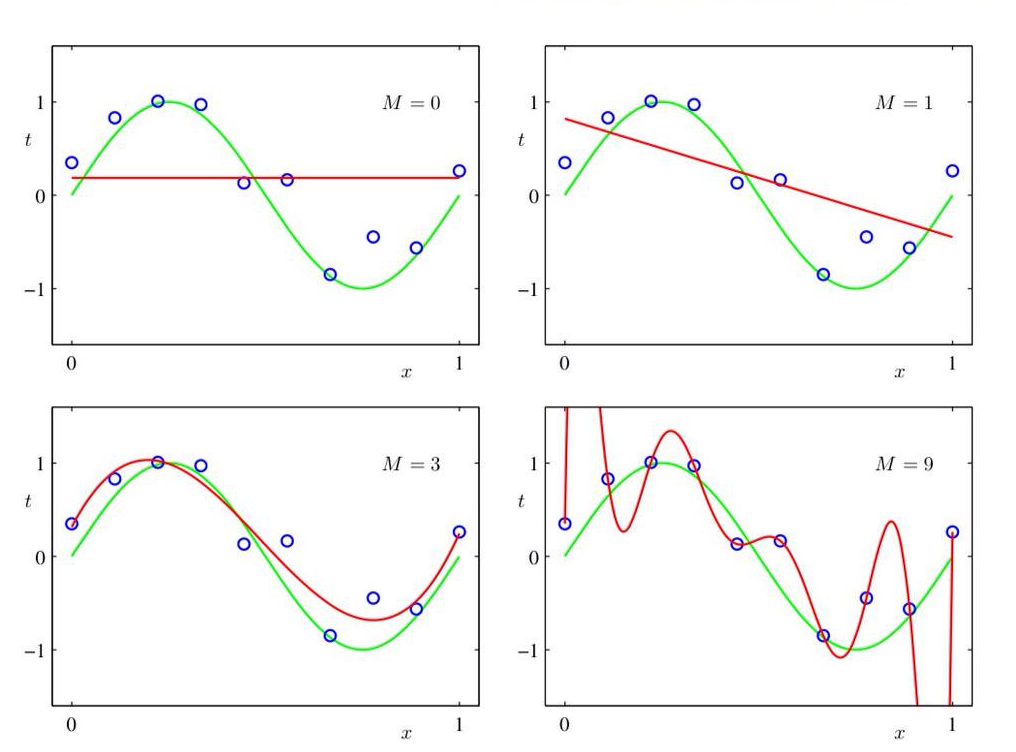
\includegraphics[height=9cm]{overfit.png}\\[0.5cm] 
\caption{Overfitting picture from Christopher M. Bishop "Pattern Recognition and Machine Learning"}
\end{figure}

The main reason for the overfitting is that the model is too complex for the dataset it is trained on. And there are a lot of different solutions to overcome this problem:
\begin{itemize}
    \item Simplify the model
    \item Greatly increase the dataset
    \item Data augmentation
    \item Cross-validation
    \item Add regularization
    \item Dropout
    \item Other techniques that improve predictions on the test or unobserved data
\end{itemize}

In the terms of the RL agent, if the agent overfits that means that he cannot perform on the states that he did not see during training. Usually, agents are trained on the same environments on which they are applied further, it means that they train on the test set. And if the environment will change or if we want to use the agent's knowledge on a similar environment (with some differences) then usually the agent will fail. A good example is the maze environment: agent can learn how to go through the maze to the finish, but when the maze will change then the agent will fail. 

This is a big problem for AGI creation, as compared to the human, a human can easily apply experience received from the one task to many other different tasks because a human can generalize. He can understand the main patterns that are important for the specific setup and then reuse this pattern in similar situations with some differences. That is why this project is focused on analyzing the ability of the agent to generalize.


\section{Related Work}

We have analyzed the current progress of generalization in Deep Reinforcement Learning field. There is a paper \cite{GeneralizationPaper} by Charles Packer, Katelyn Gao, Jernej Kos, Philipp Krähenbühl, Vladlen Koltun, Dawn Song from Berkeley that presented a good foundation to measure and analyze generalization. They have made an empirical study of generalization in Deep Learning. They implemented deterministic, random and extremely random environment setup to train on different environment setup and compare the performance using different algorithms. They compared vanilla deep RL algorithms with algorithms specialized for generalization task and empirically approved that training vanilla deep RL algorithm with environmental stochasticity may be more effective for generalization than specialized algorithms. We decided to continue their work and follow the presented approach. Train on Deterministic and Stochastic versions and test on Deterministic, Stochastic and Extremely Stochastic versions of the same environments. Generalization is a good performance of Stochastic and Extremely Stochastic versions.

\section{Solution}
As mentioned before, the agent will fail if the environment will look a little bit different from the one that the agent was trained on. So, first of all, we want to prove this statement. Then we will try to overcome this problem by making environment features representation more random, for example, sample the characteristics of the environment's objects from some distribution, and try to train the agent on such environment. Our hypothesis is that in such case the agent will not have the possibility to overfit as much as with the stable environment and because of that agent will generalize and perform better on such a random environment.

We follow convention from the mentioned paper \cite{GeneralizationPaper}:
\begin{itemize}
    \item D - Default (Deterministic) environment. It's a stable environment, parameters are fixed at the default values. There is no noise.
    \item R - Random (Stochastic) environment. The parameters are changing every time the environment is reset.
    \item E - Extreme. Same as R, but with a much higher variance of the parameters or the noise.
    \item DR - trained on D, validated on R
\end{itemize}

Due to the hierarchical structure of our work we have decided to break the project on the next pipeline:
\begin{itemize}
    \item Study RL and develop a Q-learning: model-free and the most basic value based learning algorithm. Test on a simple environment like Frozen Lake from OpenAI Gym. `Q-learning FrozenLake.ipynb` file \cite{Project}.
    \item Use DQN from OpenAI Baselines Github to train the model on the CartPole environment. It is not possible to use Q-learning for such environment as it has continuous state/action space. Train on Default and test on Default - DD.
    \item Use the environment with random and extremely random parameters (sunblaze environments \cite{Sunblaze}) to validate the poor performance of the trained DQN - DR, DE.
    \item Retrain the agent on the R environment and validate on other types - RD, RR, RE. `DQN\textunderscore for\textunderscore Sunblaze\textunderscore CartPole\textunderscore (DRE),\textunderscore openai\textunderscore baseline.ipynb` file \cite{Project}.
    \item CartPole uses only 4 features as the input, that is why we will go further and apply the same approach to the Pong (Atari game) using the state represented by pixels.
    \item Modify Pong environment so the noise can be added to the picture, modify DQN so it can be trained on the new environment with the noise.
    \item Apply the same approach of train-test as for CartPole: first DD, DR, second RD, RR. `Pong\textunderscore game\textunderscore play.ipynb` file \cite{Project}.
\end{itemize}

For training the DQN on more complex environment represented by pixels we have moved our training to the Cloud (AWS) to train using modern GPUs.

Also, the first implementation of adding noise to the environment took around 0.01 seconds to add noise to one image and it resulted to about 3 additional hours of training of the DQN as training on the simple Atari environment requires at least 1 million frames. That is why we improved the algorithm to add noise 30x times faster to not affect training time dramatically.

\section{Evaluation}

\subsection{CartPole}

\begin{figure}[H]
\centering
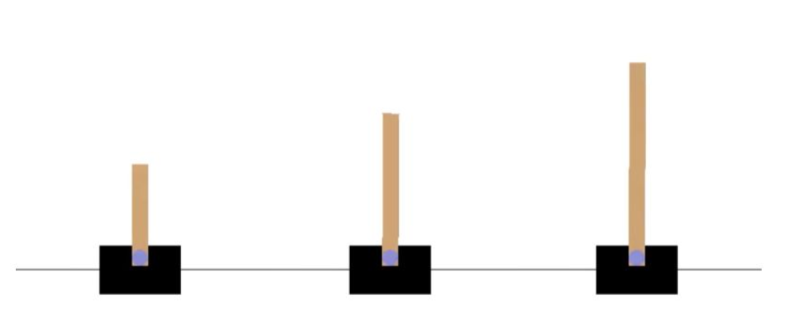
\includegraphics[height=5cm]{CartPole.png}\\[0.5cm] 
\caption{CartPole}
\end{figure}

As was expected DQN trained in the D environment has bad performance on the R and E environment. The model was training on CPU for around 45 minutes.

\begin{figure}[H]
\centering
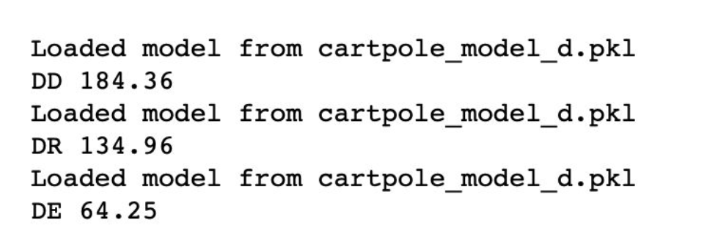
\includegraphics[height=5cm]{CartPole_bad_results.png}\\[0.5cm] 
\caption{CartPole DD, DR, DE showing poor results on the stochastic environment}
\end{figure}

After we trained an agent on the R environment, the agent performed much better on the R and E environment. The model was training on CPU for around 45 minutes.

\begin{figure}[H]
\centering
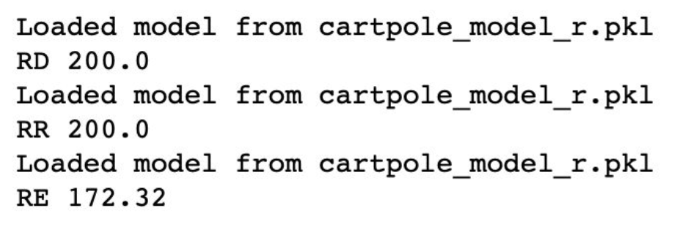
\includegraphics[height=5cm]{CartPole_good_results.png}\\[0.5cm] 
\caption{CartPole RD, RR, RE showing good results on the stochastic environment}
\end{figure}

\subsection{Pong}

\begin{figure}[H]
\centering
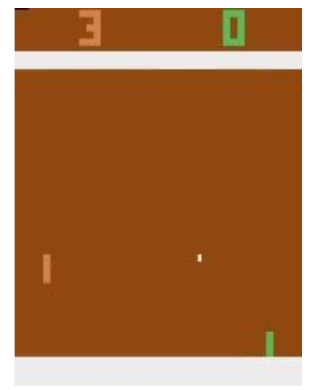
\includegraphics[height=5cm]{Pong.png}\\[0.5cm] 
\caption{Pong}
\end{figure}

We added a function that adds stochasticity to the environment.

\begin{figure}[H]
\centering
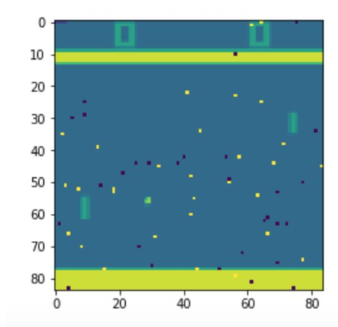
\includegraphics[height=5cm]{Pong_stochasticity.png}\\[0.5cm] 
\caption{Pong environment with stochasticity}
\end{figure}

Training agent on the D environment took 2 hours on the NVidia Tesla P100 (AWS instance). The agent performed well on D and very bad on R. After that we trained an agent on the R environment and it took around 5 hours. The second agent performed very well on D and R environments.

\begin{figure}[H]
\centering
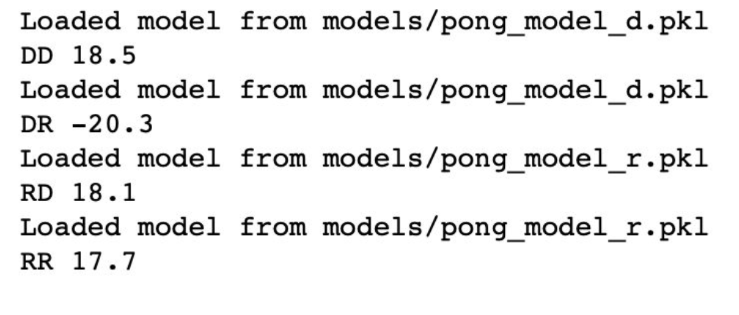
\includegraphics[height=5cm]{Pong_results.png}\\[0.5cm] 
\caption{Pong results}
\end{figure}

\section{Conclusions}

Our hypothesis was that an agent that is trained on a stable environment will have poor performance on the environment with stochastic objects and noise. We empirically approved our hypothesis on two environments with different interaction approach: we obtained the same results on CartPole environment with 4 features and Pong environment with 84x84 pixels features. Also, the same result was approved in "Assessing Generalization in Deep Reinforcement Learning" paper \cite{GeneralizationPaper}. The training procedure is much more important than complicated algorithms. Creating a stochastic environment with noise improves the ability of the agent to generalize and perform better in such environments.

\section{Future Work}

Despite that fact that we received good results improving generalization of the agent, there is still a lot of work to be done in the generalization direction to achieve a human level. A lot of more studies can be made using the current result and improving it:
\begin{itemize}
    \item Try to learn in the deterministic environment and continue to learn in the stochastic environment to reduce training duration
    \item Try different stochasticity adding not only noise but making changes in some environment rules leaving the same best policy to force an agent to learn behavior patterns instead of overfitting on some states and try to apply it on CoinRun OpenAI environment for generalization quantification \cite{CoinRun}
    \item Add stochasticity to the self-driving car virtual environment to improve agent performance when it will be transferred to the real environment
    \item Reuse agent's knowledge and experience from one environment in another having similar behavior patterns in similar situations
\end{itemize}

\newpage
\printbibliography
\end{document}